\documentclass[11pt,a4paper]{article}
\usepackage[utf8]{inputenc}
%\usepackage{ucs}
\usepackage{amsmath}
\usepackage{amsfonts}
\usepackage{amssymb}
\usepackage{graphicx}
\usepackage{listings}
\usepackage{hyperref} 
\newcommand{\opal}{\textsc{OPAL}}

\setlength{\textheight}{20.5cm}%{23.5cm}
\setlength{\oddsidemargin}{1cm}
\setlength{\textwidth}{14cm}
\setcounter{tocdepth}{2}

\author{Stefan Pauli}
\title{Bachelor Thesis\\ 
Short-range Wakefield Model Implementation in OPAL}

\newcommand{\Prob}{\mathsf{P}}  % Probability
\newcommand{\red}[1]{\stackrel{#1}{\rightarrow}}        % Reduction
\newcommand{\id}{\mathrm{id}}   %identity
\newcommand {\sign}{\mathop {\rm sign}}

\usepackage{texdraw}
\usepackage{rotating} 


\begin{document}
\maketitle
\begin{center}
\begin{tabular}{ l l }
\large Supervisors: & Dr. A. Adelmann \\
  & Prof. Dr. P. Arbenz\\
\end{tabular}
\end{center}
\mbox{}\\ \mbox{}\\ \mbox{}\\ \mbox{}\\ \mbox{}\\ \mbox{}\\ \mbox{}\\ \mbox{}\\ \mbox{}\\ \mbox{}\\ \mbox{}\\ \mbox{}\\ \mbox{}\\ \mbox{}\\ \mbox{}\\ \mbox{}\\ \mbox{}\\ \mbox{}\\ \mbox{}\\ \mbox{}\\ \mbox{}\\ \mbox{}\\ \mbox{}\\ \mbox{}\\ \mbox{}\\ \mbox{}\\ \mbox{}\\ 
ETH Zürich\\
Inst. of Computational Science
\thispagestyle{empty}
\newpage

%%\abstract
\section*{Abstract}

The Paul Scherrer Institut (PSI) is planning a new X-ray free electron
laser (XFEL).  Complex simulations must be done before constructing this
machine.  The Object Oriented Particle Accelerator Library (\opal) is
used for accurate 3D simulations.  To that end, new features have to be
introduced into OPAL.  One of them are short range wakefields, the topic
of this bachelor thesis.  First a stand alone prototype was built,
documented and tested against an already existing Mathematica notebook.
After having passed the tests the prototype was incorporated into OPAL.
\thispagestyle{empty}
\newpage
%% The Paul Scherrer Institut (PSI) is planning a new X-ray free electron
%% laser (XFEL).  Complex simulations must be done before constructing this
%% machine, among others, \opal\ (Object Oriented Particle Accelerator
%% Library) is used for 3D precise simulations. Therefore several new
%% features have to be implemented in \opal. One of them are short range
%% wakefields.

%% In this bachelor thesis short range wakefields are implemented in \opal.
%% First a stand alone prototype was made, documented and tested against a
%% already existed Mathematica notebook. After passed tests this prototype
%% was ported to \opal\ and tested again. The result of this bachelor
%% thesis is now part of \opal.
%%\newpage
\tableofcontents
\thispagestyle{empty}
\newpage
\section{Introduction}
The goal of this bachelor thesis was to add short range geometric wakefields to the Object Oriented Parallel Accelerator Library (\opal). 

\subsection{Short Range Wakefields}
%[AA a nice picture could make the description a bit more understandable] 
In special cases of physics of linear accelerators and storage rings one can consider particles at almost speed of light. This leads to the concept of wakefields and wake potentials. In this concept particles are considered as point charges moving at a velocity close to the velocity of light. If such a point charge would move in the free space, its electric and magnetic field would lie nearly in a plane passing through the charge and perpendicular to its path. This can be shown in a laboratory frame. This means that a second particle which follows the first one with the same velocity on a parallel path  will not be subjected to any forces from the fields produced by the first one. But in a linear accelerator or in a storage ring the particles are surrounded by a beam pipe, which changes the boundary conditions of those two charges. In this configuration the first particle will  not be subjected to any forces from the fields produced from the second one, because of causality. But the trailing charge feels indirectly the field of the wavefront moving with the leading charge. Because the wavefront from the first particle will be scattered at the boundary. This scattered radiation will reach the second charge and exert a force parallel and perpendicular to its direction of motion. This scattered radiation are called wakefields. The integrated effect of these wakefields over a given path length of the trailing charge is called longitudinal and transversal wake potential. One way of computing the wakefield and the forces acting on the charges due to the wakefield has been implemented in \opal\ in the framework of this the bachelor thesis. 

\subsection {\opal}
\opal\ has been developed at PSI and is used to track particles in a variety of accelerators, including cyclotrons and linear accelerators. The official homepage of \opal\ (\url{http://amas.web.psi.ch}) describes \opal\ as follows: 
"\opal\ (Object Oriented Particle Accelerator Library) is a C++ framework for general particle accelerator simulations. It includes various beam line element descriptions and methods for single particle optics, namely maps up to arbitrary order, symplectic integration schemes and lastly time integration. \opal\ is based on IPPL (Independent Parallel Particle Layer) which adds parallel capabilities. Main functions inherited from IPPL are: structured rectangular grids, fields and parallel FFT and particles with the respective interpolation operators. Other features are, expression templates and massive parallelism (up to 8000 processors) which makes is possible to tackle the largest problems in the field."

\subsection{Importance of Wakefields in PSI Simulations}
The main reason to include wakefields into \opal\ is the necessity to simulate them for the new X-ray free electron laser (XFEL). This is a linear accelerator. Ther operates with very high peak currents i.e. the particle bunch is very dense. The denser the particle bunch is, the bigger is the force due to the wakefield. Therefore, to get reliable results when simulating the new XFEL wakefields nead to be included. 
 



\section{Wakefield Calculation}

\subsection{Analytical Computation of Wakefields}
\label{sec:analytically_W_Calc}
By inverse  FFT of the beam pipe impedance the wake function is determined. For special geometries of the beam pipe analytical results of its impedance are known. The round, metallic beam pipe with radius $a$ is one example of a known impedance. There exist models of beam pipes with dc conductivity and models for ac conductivity. The dc conductivity of a metal is given by $\sigma = ne^2\tau/m$ with $n$ the density of conduction electrons, $e$ the electron charge, $\tau$ the relaxation time, and $m$ the electron mass. The ac conductivity, a response to applied oscillation fields, is given by $\tilde{\sigma} = \frac{\sigma} {1-i\omega\tau}$ with $\omega$ the frequency of the fields. According to~\cite{wake} the longitudinal impedance with dc conductivity is given by
\begin{equation}  \label{eq:Z[2]}
 Z_{Ldc}(k) = \dfrac{1}{ca} \dfrac{2}{\frac{\lambda}{k}-\frac{ika}{2}}
\end{equation}
where
\begin{equation}
\lambda=\sqrt{\dfrac{2\pi\sigma |k|}{c}}(i+\sign(k))
\end{equation}
with $c$ the speed of light and $k$ the wave number. From~\cite{notebook} a Mathematica notebook for calculating the impedance is given. Inserting $Z_0=\frac{4\pi}{c}$ and $a$ (in units of $mm$) in equation~\eqref{eq:Z[2]} leads to the form of the dc impedance in~\cite{notebook}:
\begin{equation}
  Z_{Ldc}(k) = \dfrac{Z_0}{2\pi10^{-3}a} \left( \dfrac{ \sqrt{\dfrac{\sigma Z_0|k|)}{2}} (i+\sign(k))}{k} -\dfrac{ik10^{-3}a}{2}\right)^{-1}.
\end{equation}
This has the advantage that numerical results are available to compare the own results.
The ac Impedance is given by~\cite{notebook}
\begin{equation} \label{eq:AC_Imp}
Z_{Lac}(k) = \dfrac{Z_0}{2\pi10^{-3}a} \left(\dfrac{ \sqrt{\dfrac{Z_0|k|)}{2}} \sqrt{\dfrac{\sigma}{1-ick\tau}} (i+\sign(k))} {k} -\dfrac{ik10^{-3}a}{2}\right)^{-1}.
\end{equation}
One can obtain the longitudinal wake by an inverse Fourier transformation of the impedance. Since $Re(Z_L(k))$ drops at high frequencies faster than $Im(Z_L(k))$ the cosine transformation can be used to calculate the wake. This equation holds for the dc and the ac case.
\begin{equation} \label{eq:Calc_Wl}
W_L(s)=10^{-12} \dfrac{2c}{\pi}Re\left(\int_0^\infty Re(Z_L(k))\cos (ks)dk\right)
\end{equation}
with $Z_L(k)$ either $Z_{Ldc}(k)$ or $Z_{Lac}(k)$ dependent whether the dc or the ac case is used.

The Panofsky-Wenzel theorem states
\begin{equation}
Z_L(k) = \frac{k}{c}Z_T(k).
\end{equation}
Inserting the Panofsky-Wenzel theorem in equation~\eqref{eq:Calc_Wl} the transversal wakefield reads
\begin{equation} \label{eq:Calc_Wt}
W_T(s)= 10^{-12} \dfrac{2c}{\pi}Re\left(\int_0^\infty Re( \frac{c}{k}Z_L(k))\cos (ks)dk\right).
\end{equation}

\subsection{Numerical Computation of Wakefields}
\begin{figure}[htb]
\begin{center}
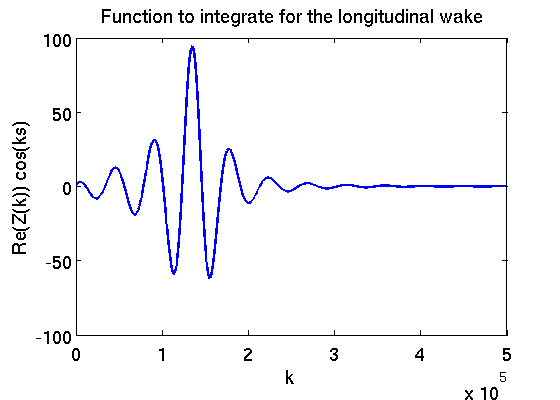
\includegraphics[width=0.7\textwidth]{wakeComp/lo_Integration.png}
\caption{The important part of the integration lies between k=0 and k=300000 \label{fig:lo_calc} }
\end{center}
\end{figure}
\begin{figure}[htb]
\begin{center}
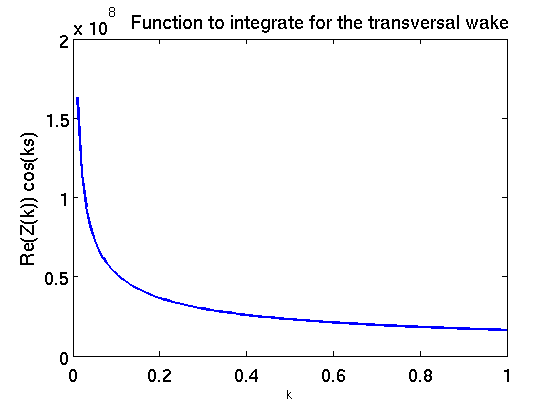
\includegraphics[width=0.7\textwidth]{wakeComp/tr_Integration.png}
\caption{A small $\Delta k$ is required to integrate this function \label{fig:tr_calc} }
\end{center}
\end{figure}

As shown in equation~\eqref{eq:Calc_Wl} and~\eqref{eq:Calc_Wt} one needs to integrate a function to calculate one sampling point of the wakefunction.
  For the numerical integration equation~\eqref{eq:Calc_Wl} is written as a sum from 0 to $N-1$ since $\infty$ can not be covered numerically, and a discrete $\Delta k$ instead of a infinitesimal $dk$:
\begin{equation}\label{eq:Num_Calc_Wl}
W_{L}(s)=10^{-12} \dfrac{2c}{\pi}Re\left(\sum_{i=0}^{N-1} Re(Z_{L}(i \Delta k))\cos (i\Delta ks)dk\right)
\end{equation}
with $Re(Z_{L})$ either $Z_{Ldc}$ or $Z_{Lac}$.
The same holds for equation~\eqref{eq:Calc_Wt} which is then writen as
\begin{equation}\label{eq:Num_Calc_Wt}
W_{T}(s)=10^{-12} \dfrac{2c}{\pi}Re\left(\sum_{i=0}^{N-1} Re(\frac{c}{k} Z_{L}(i \Delta k))\cos (i\Delta ks)dk\right).
\end{equation}
To have reliable results out of equation~\eqref{eq:Num_Calc_Wl} and~\eqref{eq:Num_Calc_Wt} $N$ the number of sampling points must be big enough and $\Delta k$ the mesh size small enough.
Figure~\eqref{fig:lo_calc} and Figure~\eqref{fig:tr_calc} give an indication how to choose $N$ and $\Delta k$. in both figures the parameters are chosen for a round, copper beam pipe with radius 5 mm. In figure~\eqref{fig:lo_calc}  $Re(Z_{Ldc}(k))\cos (ks)$ with $s$=120 $\mu$m is plotted with respect to k. This equation is integrated in equation~\eqref{eq:Num_Calc_Wl} to get the longitudinal wakefield. There it is obvious that k must be at least in the order of $10^5$. In figure~\eqref{fig:tr_calc} $Re(\frac{c}{k}Z_{Lac}(k))\cos (ks)$ with $s$=120 $\mu$m is plotted with respect to k. This equation is integrated according to equation~\eqref{eq:Num_Calc_Wt} to get the transversal wakefield. Figure shows a singularity at k=0. To integrate such functions a small $\Delta k$ (fine mesh) is needed. To simplify the understanding and the implementation of the code it would be nice to have the same integration schema for both wakes. In this bachelor thesis the Simpson integration schema with equidistant mesh size was used. This leads to an integration with small  $\Delta k$ with a big $N$ which is computational not so efficient. Since the calculation of the wakefield is usually just made once in the initialization phase of the program this does not hurt the performance of the program so much. \\
It would make sense to change to a schema with adaptive mesh size to improve the efficiency of the wake calculation.



\subsection{Using other Wakefields}
The application area for wakefield generated by round, metallic beam pipes with a certain radius is limited. Therefore one needs to be able to integrate in the code different wakefields leading to the possibility to simulate the behavior of particles in any kind of beam pipe.
This is solved by the possibility to load the data from any $W_L(s)$ and $W_T(s)$ in to \opal.
According to section~\ref{sec:Disc_Calc_Force}  values of $W_L(s)$ or $W_T(s)$ are just needed at several discreet points for s to calculate the force on the particle. If the data loaded in to opal does not provide the function values at those points, the function values are interpolated in a linear way.
This makes it possible to calculate in external programs any kind of wakefields and load them in to \opal. Hence simulations can be done with any kind of beam pipes.

\subsection{Calculate the Force on the Particles}
\label{sec:Calc_Force}

If one has the line density $\lambda$ of the particle bunch and the wakefield one can compute a force acting on the particle. The wakeforce parallel to the direction of motion of the particle can be calculated using equation~\eqref{eq:F_x}, the force perpendicular to its direction of motion can be computed using equation~\eqref{eq:F_y} and~\eqref{eq:F_z} given by~\cite{impact}.
\begin{equation} \label{eq:F_x}
F_x(s) = q\int_0^\infty W_T(s-s')x(s')\lambda(s')ds'
\end{equation}
\begin{equation} \label{eq:F_y}
F_y(s) = q\int_0^\infty W_T(s-s')y(s')\lambda(s')ds'
\end{equation}
\begin{equation} \label{eq:F_z}
F_z(s) = q\int_0^\infty W_L(s-s')\lambda(s')ds'
\end{equation}
with z parallel to the direction of motion of the particle, x(s) the shortest distance between the center of the beam pipe and the particle in x direction and y(s) the shortest distance between the center of the beam pipe and the particle in y direction.


\subsubsection{Discrete Calculation of the Force}
\label{sec:Disc_Calc_Force}
In the simulation space an time are discrete. Hence space is divided in finite slice. Particles being in the same slice feel the same force. Therefore it is reasonable to calculate the force exert for every slice. This calculation is called energy spread in~\cite{notebook}.

Space discrete signals are used to write equation~\eqref{eq:F_x} to~\eqref{eq:F_z} in a discrete form. Signals in the from $x[n]$ are defined as $x[n] = x(s)\mid_{s=n\Delta s}$.
\begin{equation} \label{eq:F_x_disc}
F_x[n] = q\sum_{i=0}^{N-1} W_T[n-i]x[i]\lambda[i]
\end{equation}
\begin{equation}
F_y[n] = q\sum_{i=0}^{N-1} W_T[n-i]y[i]\lambda[i]
\end{equation}
\begin{equation}
F_z[n] = q\sum_{i=0}^{N-1} W_L[n-i]\lambda[i].
\end{equation}
A convolution can be calculated with FFT and IFFT with $\mathcal{O}(n \log n)$ instead of $\mathcal{O}(n^2)$. Therefore it is a goal to bring those equations in the form of a convolution $y[n] = \sum_{i=-N}^{N} a[n-i]b[i]$.
This can be achieved with th Heaviside step function \begin{equation} H[n]=\begin{cases}
  0,  & n<0\\
  1, & n\geq 0
\end{cases}\end{equation}
where the equations can be written as
\begin{equation}
F_x[n] = q\sum_{i=-N+1}^{N-1} W_T[n-i]H[n-i]x[i]\lambda[i] H[i]
\end{equation}
\begin{equation}
F_y[n] = q\sum_{i=N+1}^{N-1} W_T[n-i]y[i]\lambda[i] H[i]
\end{equation}
\begin{equation}
F_z[n] = q\sum_{i=N+1}^{N-1} W_L[n-i]\lambda[i]H[i].
\end{equation}
Using FFT this lead to the form implemented in the program. The transformation pair is written as
\begin{equation}
\vec{F_x} = q\text{IFFT}(\text{FFT} (\vec{W_T}) \text{FFT}(\vec{x}\vec{\lambda}\vec{H})
\end{equation}
\begin{equation}
\vec{F_y} = q\text{IFFT}(\text{FFT} (\vec{W_T}) \text{FFT}(\vec{y}\vec{\lambda}\vec{H})
\end{equation}
\begin{equation}
\vec{F_z} = q\text{IFFT}(\text{FFT} (\vec{W_T}) \text{FFT}(\vec{\lambda}\vec{H})
\end{equation}
where for all signals holds $\vec{x} = \{x[-N+1], x[-N] ,\cdots , x[N-1]\}$.







\section{Build a Prototype}
Our prototype is a stand alone application which calculates wakefields and computes the resulting forces on the particle. 

\subsection{Why a Prototype}
According to the \opal\ doxygen documentation \opal\ consist of 842 program files and has 492 classes. This gives a rough idea how complex and big \opal\ is. To get to know such a huge program takes a while. To learn in the same time things about wakefield and implementing them would be to much. Therefore it made sense to partition those topics in different steps. One good way is to first make a stand alone application which implements most of the tasks of this bachelor thesis. Towards the end of the bachelor thesis this prototype can be ported to opal. In this way one can first understand, implement and test the wakefunction without the complexity of opal. Afterwards by the implementation in \opal\ the complexity is reduced since one has a already tested program to port to \opal.

\subsection{Approach}
First a Prototype was implemented in MATLAB. This has the advantage that it is quite fast coded and that one can make plots of everything very easy. After the MATLAB Prototype was validated (see section~\ref{sec:Val_Prototype}) a prototype in C++ was made. Since \opal\ is also written in C++ this prototype will be well portable to \opal.

\subsection{Functionality of the Prototype}
\subsubsection{Calculate the wakefield}
Calculating the wakefield of a round, metallic beam pipe was the first task of the prototype. In section~\ref{sec:analytically_W_Calc} the needed functions are given for bough the transversal and the longitudinal wakefield. In the prototype one can choose between a copper and a aluminum beam pipe with arbitrary radius. This is enough for testing the prototype, but one could easily expansion this to other materials.
\subsubsection{Calculate the Force}
The next implemented functionality is the calculation of the force acting on the particles. The equations are given in section~\ref{sec:Calc_Force}. In this equations a particle line density $\lambda$ is used. In the prototype one need to assume a particle density. Since the space is discretized particles being in the same slice feel the same force. Therefore it is reasonable to calculate the force exert for every slice. This calculation is called energy spread in~\cite{notebook}.

This calculation of the force will be made in opal in every step. Therefore it is very important to make the computation of the force as chap as possible. As discussed in section~\ref{sec:Disc_Calc_Force} the force can be calculated using FFT. This takes only $\mathcal{O}(n \log(n))$ instead of $\mathcal{O}(n^2)$ computation effort.
\subsubsection{Two Particle Model}
\label{sec:Two_Particle_Model}
The Leap Frog algorithm is used to implement the two particle model. One of
those two particle is the whole particle bunch and the other particle is a
single particle. The bunch is just negligible influenced by the single
particle. For this reason just the force on the single particle is
calculated. Therefore the form of the bunch does not change, and all the
particles from the bunch have a constant velocity of $\beta$. The velocity of
the single particle is time variant. Therefore an integration method is used to calculate position and velocity of the single particle after a certain time $t$. To conserve energy the Leap Frog algorithm is chosen. \\
This calculation of the new position of a particle can be done seperatly for all start positions of the particle. Then a plot is provided with all this particle position relative to the particle position without wakefields. This functionality is only integrated in the MATLAB code.

\subsection{Documentation}
A proper documentation is required if a code should be useful for other persons. To make live easy for the user the documentation should use standard formats. In MATLAB it is common that you can access to the documentation with typing help filename in the command window. In C++ doxygen documentation is common and also used in opal. Therefore those documentation forms were chosen. The documentation of the code is only made there. Hence there is no code documentation in this document. To give a short idea how the documentation looks like here two examples, one for MATLAB and one for the C++ code.
 \begin{figure}[htb]
\begin{center}
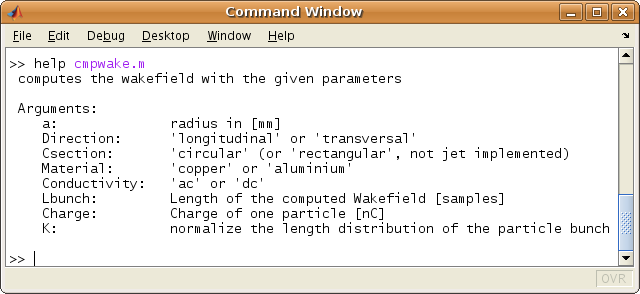
\includegraphics[width=1\textwidth]{codDoc/mat_doc.png}
\caption{Example of the MATLAB prototype documentation \label{fig:mat_doc} }
\end{center}
\end{figure}
\begin{figure}[htb]
\begin{center}
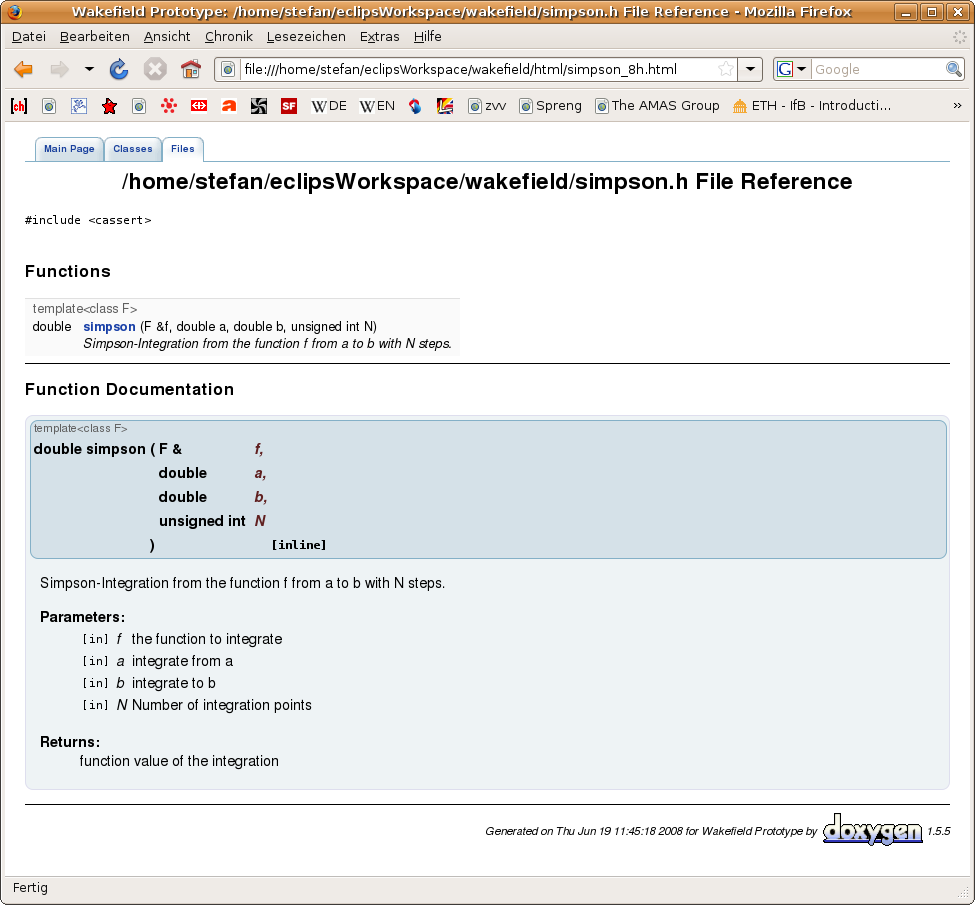
\includegraphics[width=1\textwidth]{codDoc/cpp_doc.png}
\caption{Example of the C++ prototype documentation \label{fig:cpp_doc} }
\end{center}
\end{figure}
Figure~\ref{fig:mat_doc} shows the result when typing help cmpwake.m in the MATLAB command window. Figure~\ref{fig:cpp_doc} shows a example of the C++ code documentation.

\clearpage
\section{Validation of the Prototype}
\label{sec:Val_Prototype}
 \subsection{Comparison with the Mathematica code}
One way of validating the prototype is to compare its results with the results of an existing Mathematica code~\cite{notebook}. This Mathematica code computes a wakefield and a energy spread. For comparison the energy spread an the wakefield are compared with different settings.


\begin{figure}[htb]
\begin{center}
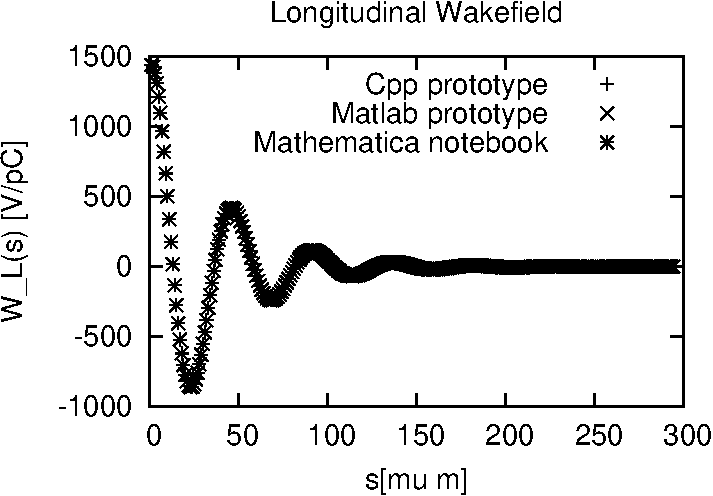
\includegraphics[width=0.6\textwidth]{wakeCompare/wake_Lo_Circ_Cu_AC_5.pdf}
\caption{Comparison of the MATLAB and the C++ prototype with the Mathematica code from~\cite{notebook}. This is the longitudinal wakefunktion of a round, copper beam pipe with radius 5 mm and ac conductivity. \label{fig:wave} }
\end{center}
\end{figure}
\begin{figure}[htb]
\begin{center}
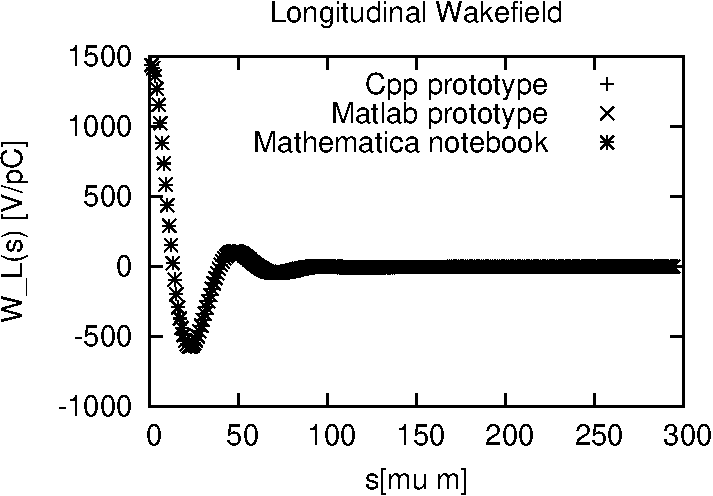
\includegraphics[width=0.6\textwidth]{wakeCompare/wake_Lo_Circ_Al_AC_5.pdf}
\caption{Comparison of the MATLAB and the C++ prototype with the Mathematica code from~\cite{notebook}. This is the longitudinal wakefunktion of a round, aluminum beam pipe with radius 5 mm and ac conductivity. \label{fig:wave_Al} }
\end{center}
\end{figure}

Figure~\ref{fig:wave} shows that the result is equal for the prototype and the Mathematica code for the longitudinal wakefield for a round, copper beam pipe with radius 5 mm and ac conductivity. This holds for all wave function tested with the 3 codes. Figure~\ref{fig:wave_Al} is a second example where the prototype agrees with the Mathematica code.

\begin{figure}[htb]
\begin{center}
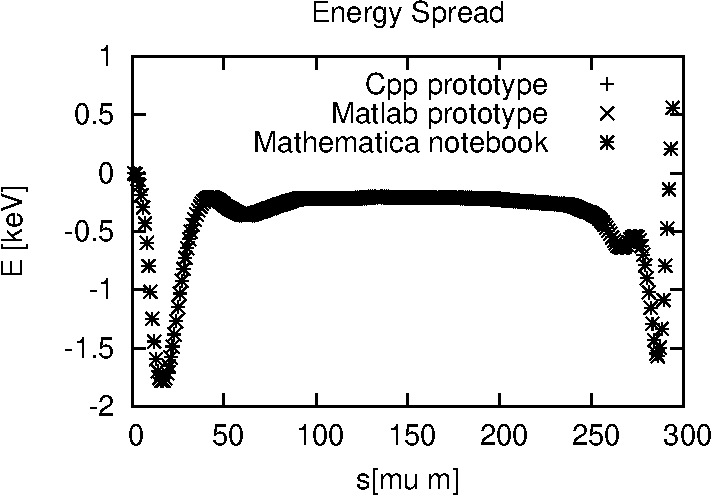
\includegraphics[width=0.6\textwidth]{wakeCompare/energy_Lo_Circ_Al_AC_5.pdf}
\caption{Comparison of the MATLAB and the C++ prototype with the Mathematica code from~\cite{notebook}. This is the so called energy spread in~\cite{notebook} resulting from a longitudinal wakefunktion of a round, aluminum beam pipe with radius 5 mm and ac conductivity with the line density $\lambda$ from~\cite{notebook}. \label{fig:energy_Al} }
\end{center}
\end{figure}
A comparison between the energy spreads of the Mathematica code and the prototype in C++ or MATLAB with always the same result can bee seen in Figure~\ref{fig:energy_Al}.
\clearpage
\section{Implementation in \opal}

The C++ prototype was ported to \opal. Hence most of the functionality is the same as in the prototype. Topics already discussed in connection with the prototype are omitted in this section to avoid repetition. New topics valid only for the implementation of \opal\ are presented in this section.  


\subsection{Parallelism}
The P in \opal\ stands for "parallelism". Therefore the new wakefunction must be parallel as well. A simple example is that cout does not work, *gmsg a \opal\ function which provides that just processor 0 writes to the shell must be used instead.
In \opal\ the particles are already distributed over several processors. Using those local particles lead to a parallel implementation of adding the force to the particles. This could not be tested, since the function calling the wakefield is not yet parallel.

\subsubsection{Adding the Force to the Particle}
In \opal\ the force due to the wakefields is not the only force acting on particles. There exist for example particle particle interaction, external electric and magnetic fields. Therefore one need to add the force due to wakefield to the already existing forces. Instead of having force as an variable opal store the E and B field at the particle and calculate the force using $F = q[\vec{E}+v\times\vec{B}]$. One can now add the force coming from the wake using $\vec{E} = \vec{E}_{coulomb} + \vec{E}_{extern} + \vec{E}_{wake}$.
Where the electric field for the particle i is:
\begin{equation} \vec{E(s(i))}_{wake} =  \left( \begin{array}{c}
 E_x(s(i))  \\  E_y(s(i))  \\  E_z(s(i))  \\
\end{array} \right)
=  \left( \begin{array}{c} F_x(s(i))/q \\  F_y(s(i))/q \\  F_z(s(i))/q
\end{array} \right).
\end{equation}

\subsection{Units}
\label{sec:units}
\opal\ uses the SI units. In the Prototype some units were not in SI units for example the radius of the beam pipe was in mm instead of m. This had to be changed in the code to have a proper running simulation in \opal.


\subsection{One of the Challenges}
Since \opal\ is very powerful the amount of code already written is impressive. In the beginning it was challenging to cope with such a program. Even a easy thing like calculating the line density of the particle bunch, which is already provided as a function and therefore just can be called, was in the beginning demanding. Therefore a good documentation is needed to find those functions and to know how to apply them.

\subsection{Documentation}
A Doxygen documentation of the whole \opal\ can be found at 
\url{http://amas.web.psi.ch}. There the documentation of the code written during the Bachelor thesis is integrated. As the C++ prototype and this code are documented with Doxygen the main part of the Doxygen comment used for the documentation could be reused from the prototype. Figure~\ref{fig:OPAL_doc} shows where the function CalcWakeFFT() is documented.
\begin{figure}[htb]
\begin{center}
\includegraphics[width=1\textwidth]{codDoc/Opal_doc.png}
\caption{Example of the documentation of the code of this bachelor thesis in \opal\ under 
\url{http://amas.web.psi.ch}   \label{fig:OPAL_doc} }
\end{center}
\end{figure}


\clearpage


\subsection{Parameters of the Wakefield}
A wakefield in \opal\ has several attributes. They are documented in the \opal\ manual. By typing help,wake; in the running \opal\ shell the attributes are printed on the screen. The result can be seen below:

\begin{verbatim}
The "WAKE" statement defines data for a the wakefunction on an element.
Attributes:
string   TYPE          Specifies the wake function: 1D-CSR, 
                       LONG-SHORT-RANGE, TRANSV-SHORT-RANGE, 
                       LONG-TRANSV-SHORT-RANGE
real     NBIN          Number of bins for the line density calculation
logical  CONST_LENGTH  True if the length of the Bunch is considered
                       as constant
string   CONDUCT       Cundivity: DC, AC
real     Z0            Impedanz of the beam pipe
string   FORM          The form of the  beam pipe: ROUND
real     RADIUS        The radius of the beam pipe [m]
real     SIGMA         Material constant dependant on the  
                       beam pipe material
real     TAU           Material constant dependant on the  
                       beam pipe material
\end{verbatim}

\subsection{Add Wakefunction to a Unit in \opal}
\opal\ provides a meta language to simulate a accelerator. In this language few programming knowledge is needed to compose and simulate a hole accelerator. The next lines should give a rough idea how this meta language works and how easy a wake function can be added to an existing part of the accelerator.
First one must specify the properties of the wake.
\begin{verbatim}
W1: Wake, TYPE="LONG-SHORT-RANGE", NBIN=10, CONST_LENGTH=true,
CONDUCT="AC", Z0=376.991118, FORM="ROUND",
RADIUS=0.005, SIGMA=6.45337e7, TAU=2.70187e-14;
\end{verbatim}
Then one can add very easy a wake function to a existing part of the accelerator, in this case to a RF Cavity. In this to lines a RF Cavity with and one without Wake is shown.
\begin{verbatim}
FINLB01_RACF: RFCavity, L=0.54, VOLT=19.961*1.641907, 
FMAPFN="FINLB01-RACF.T7", ELEMEDGE=0.069, TYPE="STANDING", 
FREQ=1498.956, LAG=184.0/360.0, Wake=W1;

FINLB01_RACH: RFCavity, L=0.54, VOLT= 6.250*1.641907, 
FMAPFN="FINLB01-RACH.T7", ELEMEDGE=0.069, 
TYPE="STANDING", FREQ=4497.536, LAG=104.0/360.0;
\end{verbatim}
The rest is the same as it would be with out wakefunction. Some of the following needed steps are shown below, to give a rough idea how easy a accelerator can be implemented. The particle beam must be specified, the single parts of the accelerator patched together, and then the beam can be tracked while going through the accelerator.
\begin{verbatim}
beam1: BEAM, PARTICLE=ELECTRON, pc=P0, NPART=5e4, 
BFREQ=1498.953425154e6, BCURRENT=0.032912, CHARGE=-1;
l1: Line = (FINLB01_RACF, FINLB01_RACH);
track,line=l1, beam=beam1, MAXSTEPS=400, DT=1.0e-12;
\end{verbatim}


\section{Validation in \opal}
\subsection{Comparison with the Prototype}
\subsubsection{Without SI Units}
As mentioned in section~\ref{sec:units} the Mathematica notebook~\cite{notebook} uses not SI units, for example mm instead of m. To avoid troubles with that, the first test in \opal\ was made using the units from the Mathematica notebook. This first test should ensure that the part which is already implemented in the prototype works. Therefore the results of the wakefield code in \opal\ was compared with the results from the prototype. To have comparable data the properties of the bunch must be simular. To ensure that, the length and the line density  of the particle bunch were taken from the prototype and programmed in to a test function. Then the \opal\ code could be tested under the same condition as the prototype. In Figure~\ref{fig:wakeOPAL} and Figure~\ref{fig:energyOPAL} both simulations give the same results. That indicates that the calculation of the wakefield and of the force works in \opal. The next step is to ensure that the simulation works correctly with the SI units used in \opal.
\begin{figure}[htb]
\begin{center}
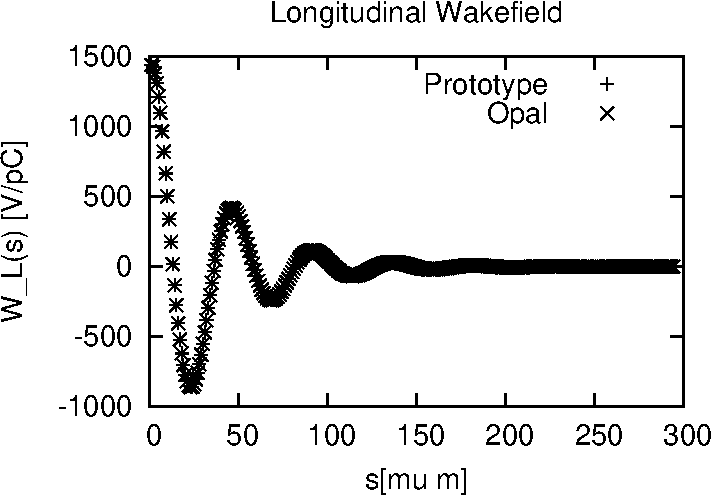
\includegraphics[width=0.6\textwidth]{wakeCompare/wake_Lo_Circ_Cu_AC_5_OPAL.pdf} 
\caption{With equal properties the Simulation in \opal\ gives the same wakefunction as the prototype. This is the longitudinal wakefunktion of a round, copper beam pipe with radius 5 mm and ac conductivity.
\label{fig:wakeOPAL} }
\end{center}
\end{figure}

\begin{figure}[htb]
\begin{center}
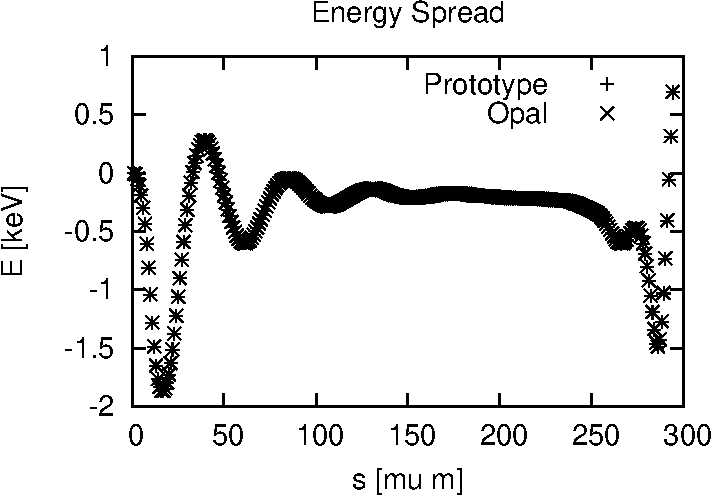
\includegraphics[width=0.6\textwidth]{wakeCompare/energy_Lo_Circ_Cu_AC_5_Opal.pdf} 
\caption{With equal properties the Simulation in \opal\ gives the same kick as the prototype. This is the so called energy spread in~\cite{notebook} resulting from a longitudinal wakefunktion of a round, aluminum beam pipe with radius 5 mm and ac conductivity with the line density $\lambda$ from~\cite{notebook}. \label{fig:energyOPAL} }
\end{center}
\end{figure}

\clearpage
\subsubsection{With SI Units}
All units are changed to SI units. To change the units is normally  quite error-prone. Therefore this test is useful. The line density used in the prototype is still used in this test to compare the results with the prototype. This test shows that aside from a constant factor the results from Opal are equal to those of the prototype. To have good possibility of comparison this factor was calculate out of the results plotted in Figure~\ref{fig:wakeOPAL_SI}. Therefore all the results of the wakefield calculated by \opal\ were multiplied by a factor of 10. The as you can see on Figure~\ref{fig:wakeOPAL_SI} the results of the wakefield computed in \opal\ give the same results as those from the prototype apart from the factor 10.

As for the wakefield the energy spread is also correct aside from a constant factor. Dividing all the results from \opal\ by a constant factor of $10^6$ the energy spread gives the same results as the prototype, as shown in Figure~\ref{fig:energyOPAL_SI}.

Unfortunately there is no time left in the my bachelor thesis to solve this problem. But i am confidently that the problem can be localized and solved quite fast.


\begin{figure}[htb]
\begin{center}
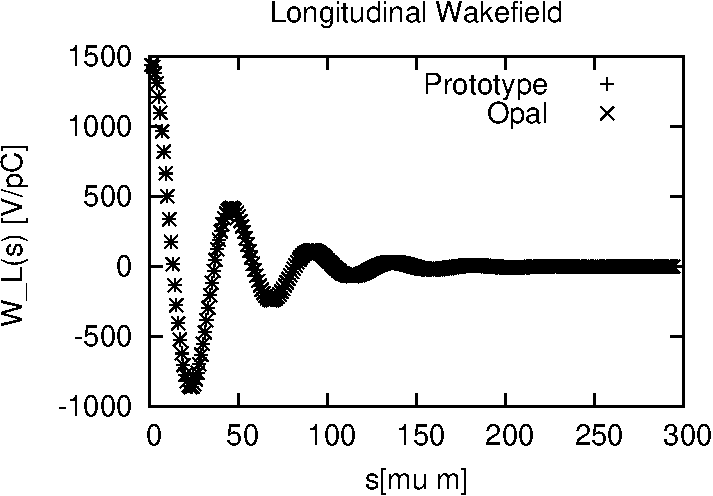
\includegraphics[width=.6\textwidth]{wakeCompare/wake_Lo_Circ_Cu_AC_5_OpalNew.pdf}
\caption{The wakefield of \opal\ is multiplied by a factor of 10. Aside from this factor the \opal\ code gives the same results as the prototype. This is the longitudinal wakefield of a round, copper beam pipe with radius 5 mm and ac conductivity.
\label{fig:wakeOPAL_SI} }
\end{center}
\end{figure}

\begin{figure}[htb]
\begin{center}
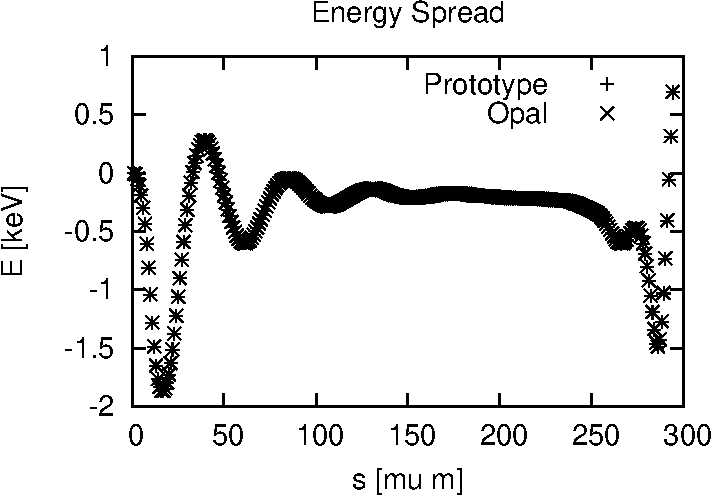
\includegraphics[width=.6\textwidth]{wakeCompare/energy_Lo_Circ_Cu_AC_5_OpalNew.pdf}
\caption{The energy of \opal\ is divided by a factor of $10^6$.Aside form this factor the \opal\ code gives the same results as the prototype. This is the energy spread in~\cite{notebook} resulting from a longitudinal wakefield of a round, copper beam pipe with radius 5 mm and ac conductivity with the line density $\lambda$ from~\cite{notebook}.
\label{fig:energyOPAL_SI} }
\end{center}
\end{figure}



\clearpage
\section{Summary}
Due to the good documentation of the wakefield implementation in \opal\ 
it should be possible to continue the work started with this bachelor
thesis. Possible next steps are presented in the following subsection.

\subsection{Outlook}
First the unsolved unit problem should be solved. Afterwards the code
can be used for simulating the new XFEL at the PSI.

The calculation of the wakefield at the program start takes quite long.
This part in not jet parallel. The parallelization of both
equations~\eqref{eq:Num_Calc_Wl} and~\eqref{eq:Num_Calc_Wt} would be
trivial. The sum over N could be calculated in parallel by p processors,
in the consequence that each processor only make a sum over
$\frac{N}{p}$. This calculation can be made without communication.
Communication is only needed to gathered the result.

A speedup could also be managed if a schema with adaptive mesh would be
used at the integration to get the wakefield.

\section*{Acknowledgment}
I would like to thank Dr. Andreas Adelmann for the agreeable mentoring
and the amas crew at the PSI for the interesting time I could spent with
them at the PSI. Finally I would like to thank Prof. Dr. Peter Arbenz
and Dr. Andreas Adelmann for giving me the chance to work on such an
fascinating topic!



\begin{thebibliography}{9}
  
\bibitem{notebook} C.~Bontoiu and P.~Craievich: How to use RW\_wakefield
  notebook.
  
\bibitem{wake} A.W.~Chao: \newblock{Physics of collective beam
    instabilities in high energy accelerators, John Wiley \& Sons, New
    York, 1993}.
   
\bibitem{impact} J.~Qiang: {\em IMPACT-T User Document Version 1.5}.
  Lawrence Berkeley National Laboratory, LBNL-62326, 2007.
 
\end{thebibliography}

\end{document}
